% vim:spelllang=ru,en
\documentclass[a4paper,12pt,notitlepage,headsepline,pdftex]{scrartcl}

\usepackage{cmap} % чтобы работал поиск по PDF
\usepackage[T2A]{fontenc}
\usepackage[utf8]{inputenc}
\usepackage[english,russian]{babel}
\usepackage{concrete}
\usepackage{cite}
\usepackage{url}

\usepackage{textcase}
\usepackage[pdftex]{graphicx}

\usepackage{lscape}

\pdfcompresslevel=9 % сжимать PDF
\usepackage{pdflscape} % для возможности альбомного размещения некоторых страниц
\usepackage[pdftex]{hyperref}
% настройка ссылок в оглавлении для pdf формата
\hypersetup{unicode=true,
            pdftitle={ПОЭВМ Лаба №3},
            pdfauthor={Погода Михаил},
            pdfcreator={pdflatex},
            pdfsubject={},
            pdfborder    = {0 0 0},
            bookmarksopen,
            bookmarksnumbered,
            bookmarksopenlevel = 2,
            pdfkeywords={},
            colorlinks=true, % установка цвета ссылок в оглавлении
            citecolor=black,
            filecolor=black,
            linkcolor=black,
            urlcolor=blue}

\usepackage{amsmath}
\usepackage{amssymb}
\usepackage{moreverb}
\usepackage{indentfirst}
\usepackage{misccorr}

\usepackage{xtab}
\usepackage{nccfoots}
\usepackage{listings}

\lstloadlanguages{C++}
\lstset{language=C++,basicstyle=\scriptsize,frame=tb,commentstyle=\itshape,stringstyle=\bfseries,extendedchars=false}
\begin{document}
\begin{titlepage}
  \begin{center}
    \large
    \MakeUppercase{Министерство образования и науки,}

    \MakeUppercase{молодёжи и спорта Украины}

    \mbox{\MakeUppercase{Национальный технический университет Украины}}

    \MakeUppercase{,,Киевский политехнический институт''}

    \addvspace{6pt}

    \normalsize
    Кафедра прикладной математики

    \vfill

    \textbf{Отчёт}

    Лабораторная работа \No 3

    по дисциплине ,,Программное обеспечение ЭВМ''

    \emph{,,Решение обычных дифференциальных уравнений''}
  \end{center}

  \vfill

  \noindent
  \begin{minipage}{0.3\textwidth}
    Выполнил

    студент группы КМ-92

    Погода~М.\,В.
  \end{minipage}
  \hfill
  \begin{minipage}{0.4\textwidth}
    Проверила:

    Ковальчук"=Химюк~Л.\,А.
  \end{minipage}
  \vfill

  \begin{center}
    КИЕВ

    2012
  \end{center}
\end{titlepage}
\tableofcontents
\newpage
\section{Постановка задачи}
  Даны:
  \begin{itemize}
    \item Дифференциальное уравнение:
      \begin{equation}
        \frac{d^2 y}{dx^2} = f\left( x, y, \frac{dy}{dx} \right)
        \label{eq:diffeq}
      \end{equation}
    \item Интервал, на котором необходимо решить~\eqref{eq:diffeq} $\left[
        a; b \right]$.
    \item Шаг $h$, с которым необходимо провести табуляцию функции;
    \item Начальные условия: $y\left( a \right) = C_1, \frac{dy}{dx}\left(
        a \right) = C_2$.
  \end{itemize}

  Необходимо:
  \begin{itemize}
    \item решить на ЭВМ уравнение~\eqref{eq:diffeq} численным методом;
    \item оценить точность полученного решения.
  \end{itemize}
\section{Входные данные}
  \hfill\emph{Вариант~11}

  \begin{itemize}
    \item Линейное дифференциальное уравнение второго порядка:
      \begin{equation}
        \frac{d^2 y}{d x^2} x^2 - 2y = 0
        \label{eq:eq1}
      \end{equation}
    \item Интервал, на котором необходимо решить~\eqref{eq:eq1} $\left[ 1.0;
        2.0 \right]$;
    \item Шаг $h = 0.1$;
    \item Начальные условия $y\left( 1.0 \right) = 0.83; \frac{d y}{d x}\left(
      1.0 \right) = 1.0$.
  \end{itemize}

  В качестве метода поиска решения линейного дифференциального уравнения
  необходимо использовать метод Рунге"=Кутты третьего порядка.
  \newpage
\section{Теоретические сведения}
  Метод Рунге"=Кутты применяется для решения задачи Коши:
  \begin{equation}
    \frac{d y}{d x} = f\left( x, y \right), y(x_0) = y_0
    \label{eq:cauchy}
  \end{equation}

  Во всех точках интервала рассчитывается значение функции с помощью
  приближённых формул:
  \begin{itemize}
    \item для метода третьего порядка:
      \begin{eqnarray}
        K_1 &=& h f\left( x_n, y_n \right)\\
        K_2 &=& h f\left( x_n + \frac{1}{3}h, y_n + \frac{1}{3}K_1 \right)\\
        K_3 &=& h f\left( x_n + \frac{2}{3}h, y_n + \frac{2}{3}K_2 \right)\\
        y_{n+1} &=&  y_n + \frac{1}{4}\left( K_1 + 3 K_3 \right)
        \label{eq:rk3}
      \end{eqnarray}
    \item для метода четвёртого порядка:
      \begin{eqnarray}
        K_1 &=&  h f\left( x_n, y_n \right)\\
        K_2 &=&  h f\left( x_n + \frac{h}{2}, y_n + \frac{1}{2}K_1 \right)\\
        K_3 &=&  h f\left( x_n + \frac{h}{2}, y_n + \frac{1}{2}K_2 \right)\\
        K_4 &=&  h f\left( x_n + h, y_n + K_3 \right)\\
        y_{n+1} &=&  y_n + \frac{1}{6}\left( K_1 + 2 K_2 + 2 K_3 + K_4 \right)
        \label{eq:rk4}
      \end{eqnarray}
  \end{itemize}

  Порядок метода --- порядок суммарной ошибки на конечном интервале.

  В случае уравнений высоких порядков с помощью замены вида
  $\frac{dy}{dx} = z$ уравнение сводится к системе уравнений первого порядка,
  которые решаются методом Рунге"=Кутты параллельно.
  \newpage
\section{Решение}
    Сравнительная таблица решения, полученного методом Рунге"=Кутты третьего
    находится в Приложении на странице~\pageref{tab:fxs}.

    График полученной функции можно увидеть в Приложении на
    странице~\pageref{fig:gui}.
\section{Описание программы}
  Программа написана на языке C++ с использованием библиотек
  Qt\footnote{\url{http://qt-project.org}} и
  Qwt\footnote{\url{http://qwt.sourceforge.net}}.

  Программа ищет численное решение заданного дифференциального уравнения
  методами Рунге"=Кутты третьего и четвёртого порядков и строит их графики.

  Пользователь может ввести необходимое количество интервалов разбиения, а
  также начальное значение производной функции.

  В результате работы программы выводит на форме графики функций, полученных в
  результате решения уравнения, а также средние абсолютные погрешности
  результата.
  \newpage
\section{Блок"=схема алгоритма}
  \begin{figure}[h!]
    \begin{center}
      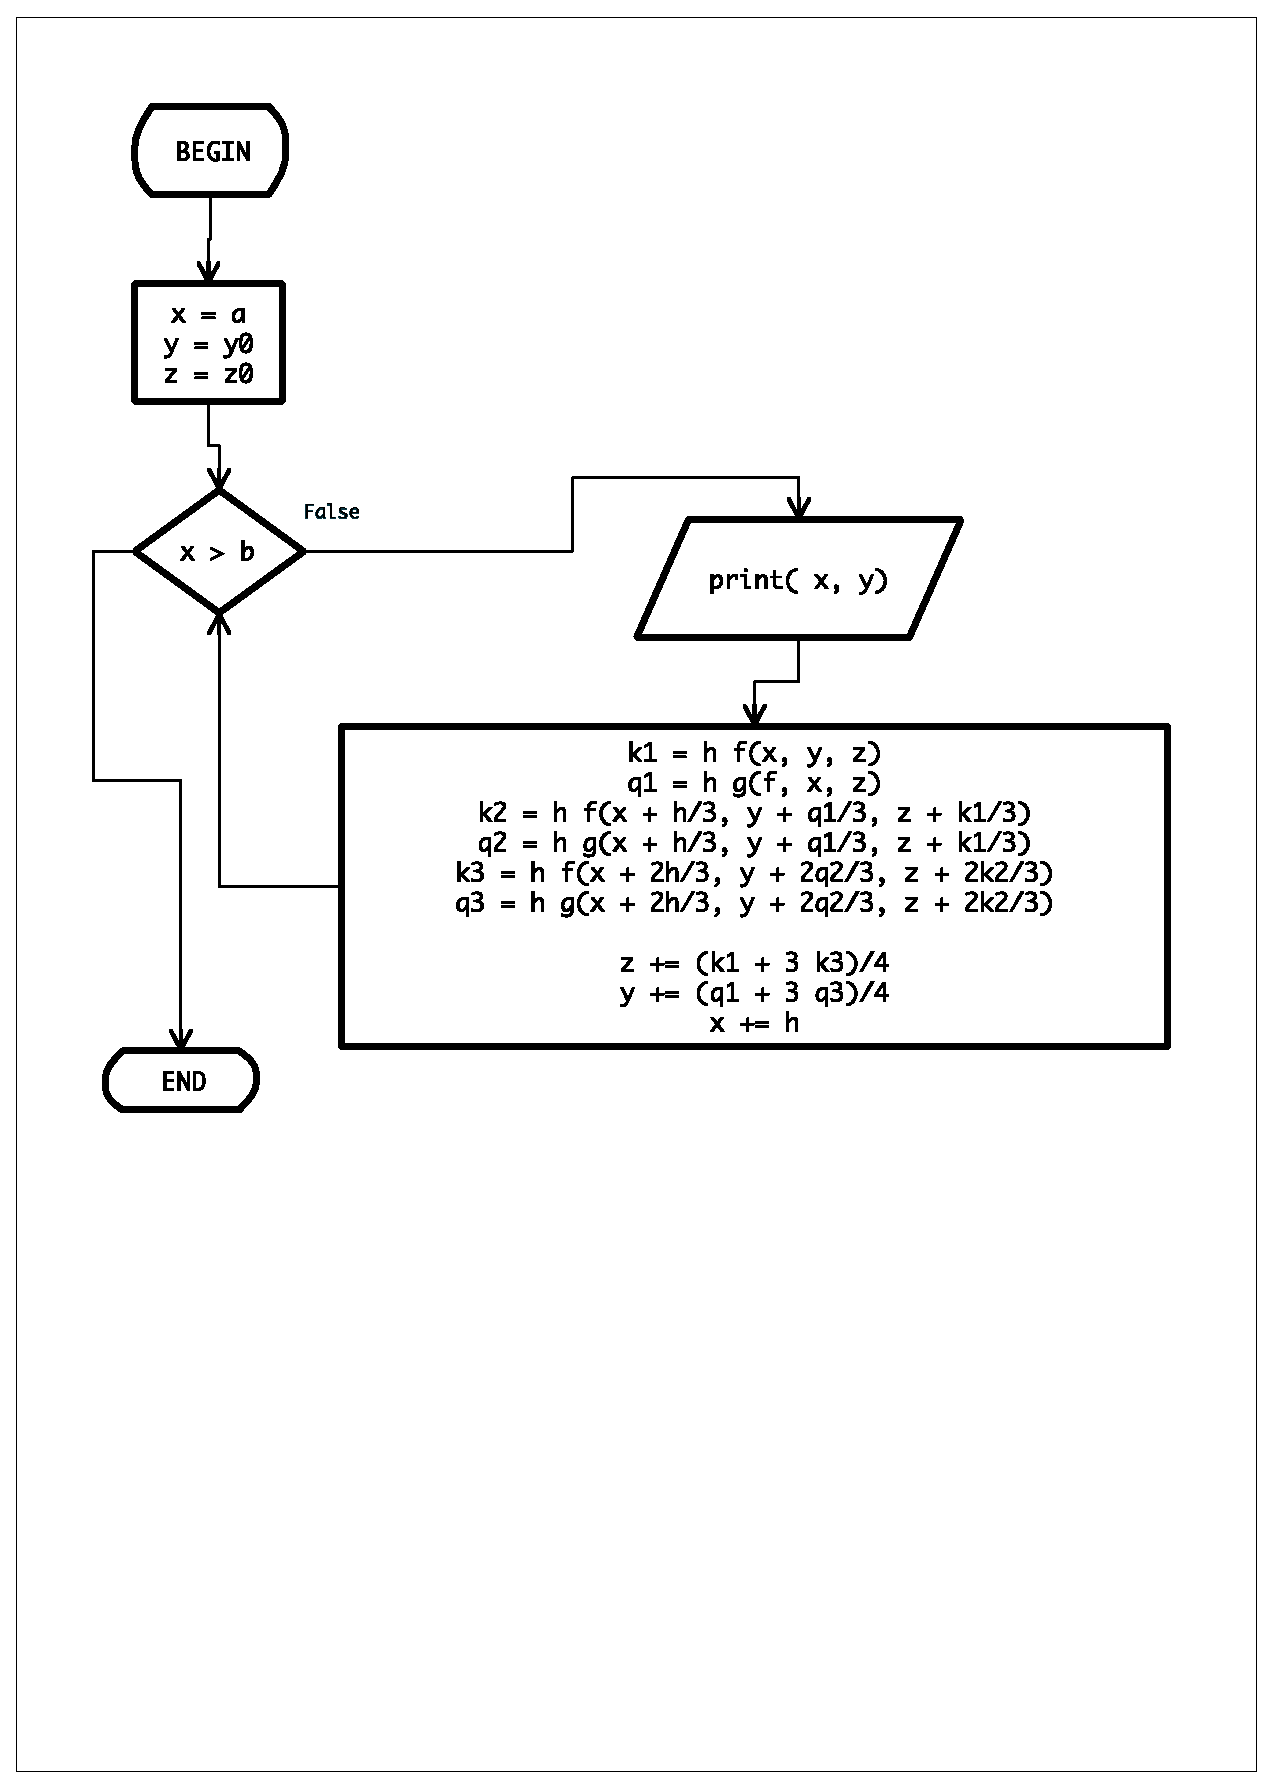
\includegraphics[scale=0.60]{flowchart.eps}
    \end{center}
    \caption{Блок"=схема алгоритма}
    \label{fig:flowchart}
  \end{figure}
  \newpage
\section{Выводы}
  При выполнении данной лабораторной работы были реализованы численные методы
  решения задачи Коши, а именно методы Рунге"=Кутты третьего и четвёртого
  порядков.

  Для поставленной задачи суммарная ошибка обоих методов не превышала
  заявленных порядков точности, а именно была равна $\approx 10^{-5}$.

  В виду этого на графики решений практически невозможно разделить визуально.
  \newpage
\section{Приложения}
  \subsection{Таблица значений полученного решения}
  \begin{table}[h!]
    \centering
    \begin{tabular}{|c|c|}
      \hline
      x & y\\
      \hline
      1.0 & 0.83\\
      1.1 & 0.94\\
      1.2 & 1.06\\
      1.3 & 1.20\\
      1.4 & 1.35\\
      1.5 & 1.52\\
      1.6 & 1.70\\
      1.7 & 1.89\\
      1.8 & 2.10\\
      1.9 & 2.32\\
      2.0 & 2.55\\
      \hline
    \end{tabular}
    \caption{Таблица значений решения}
    \label{tab:fxs}
  \end{table}
  \clearpage
  \subsection{Графическая форма приложения}
    \begin{figure}[h!]
      \begin{center}
        \includegraphics[scale=0.86]{scr.png}
      \end{center}
      \caption{Графическая форма приложения}
      \label{fig:gui}
    \end{figure}
  \subsection{Исходные тексты}
    \subsubsection{CMakeLists.txt}
      \lstinputlisting{/home/projects/apps-for-computing/lab3/CMakeLists.txt}
    \subsubsection{lab3\_widget.hxx}
      \lstinputlisting{/home/projects/apps-for-computing/lab3/lab3_widget.hxx}
    \subsubsection{lab3\_widget.cxx}
      \lstinputlisting{/home/projects/apps-for-computing/lab3/lab3_widget.cxx}
\end{document}
